\chapter{Trygonometria}
\begin{center}
  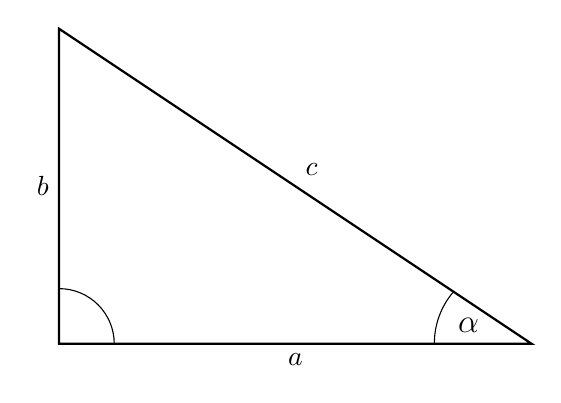
\begin{tikzpicture}
    \draw[thick] (0, 0) -- (6, 0) node[midway, below]{$a$}
    -- (0, 4) node[midway, above right]{$c$}
    -- cycle node[midway, left]{$b$};
    \draw (0.7, 0) arc (0:90:0.7);
    \draw (5, 0.65) arc (140:180:1);
    \node at (5.2, 0.23){\large$\alpha$};
  \end{tikzpicture}
\end{center}
\begin{equation}
  \begin{aligned}
    \sin\alpha &= \frac bc \qquad\qquad&\tg\alpha &= \frac ba\\[2pt]
    \cos\alpha &= \frac ac \qquad\qquad&\ctg\alpha &= \frac ab
  \end{aligned}
\end{equation}
\vspace{20pt}
\begin{center}
  \begin{tabular}{|*6{c|}}
    \hline
    & $0^\circ$ & $30^\circ$ & $45^\circ$ & $60^\circ$ & $90^\circ$\\
    \hline
    $\sin\alpha$ & 0 & $\frac 12$ & $\frac{\sqrt2}{2}$ & $\frac{\sqrt3}{2}$ & 1\\
    \hline
    $\cos\alpha$ & 1 & $\frac{\sqrt3}{2}$ & $\frac{\sqrt2}{2}$ & $\frac 12$ & 0\\
    \hline
    $\tg\alpha$ & 0 & $\frac{\sqrt3}{3}$ & 1 & $\sqrt3$ & -\\
    \hline
    $\ctg\alpha$ & - & $\sqrt3$ & 1 & $\frac{\sqrt3}{3}$ & 0\\
    \hline
  \end{tabular}
\end{center}
\section{Zależności trygonometryczne}
\begin{equation}
  \begin{aligned}
    \sin(90^\circ - \alpha) &= \cos\alpha\\
    \cos(90^\circ - \alpha) &= \sin\alpha\\
    \tg(90^\circ - \alpha) &= \ctg\alpha\\
    \ctg(90^\circ - \alpha) &= \tg\alpha
  \end{aligned}
\end{equation}
\begin{equation}
  \begin{aligned}
    \tg\alpha = \frac{\sin\alpha}{\cos\alpha}\\[4pt]
    \ctg\alpha = \frac{\cos\alpha}{\sin\alpha}
  \end{aligned}
\end{equation}
\begin{gather}
  \sin^2\alpha + \cos^2\alpha = 1\\
  \tg\alpha\cdot\ctg\alpha = 1
\end{gather}
\section{Funkcje trygonometryczne dowolnego kąta}
\begin{center}
  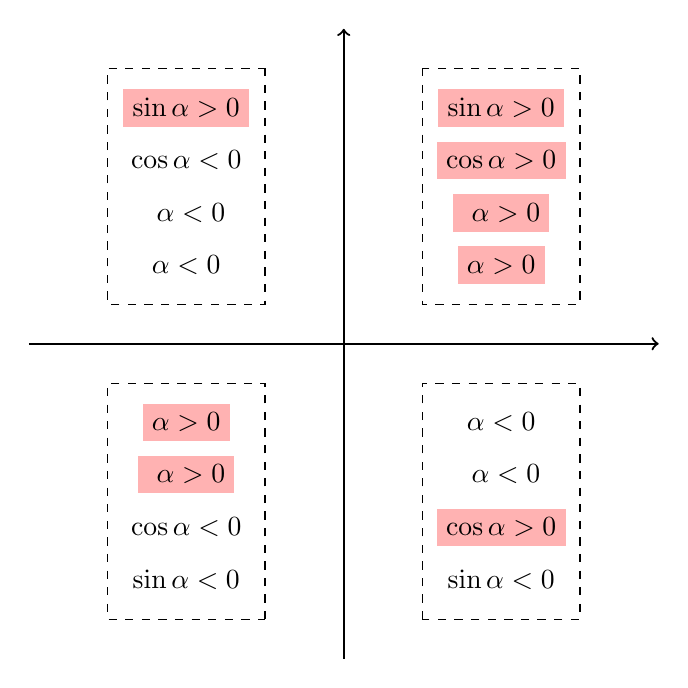
\begin{tikzpicture}
    \draw[thick, ->] (-4, 0) -- (4, 0);
    \draw[thick, ->] (0, -4) -- (0, 4);
    \draw[dashed] (1, 3.5) rectangle (3, 0.5);
    \node at (2, 3)[fill=red!30]{$\sin\alpha > 0$};
    \node at (2, 2.33)[fill=red!30]{$\cos\alpha > 0$};
    \node at (2, 1.66)[fill=red!30]{$\ \tg\alpha > 0$};
    \node at (2, 1)[fill=red!30]{$\ctg\alpha > 0$};
    \draw[dashed] (-1, 3.5) rectangle (-3, 0.5);
    \node at (-2, 3)[fill=red!30]{$\sin\alpha > 0$};
    \node at (-2, 2.33){$\cos\alpha < 0$};
    \node at (-2, 1.66){$\ \tg\alpha < 0$};
    \node at (-2, 1){$\ctg\alpha < 0$};
    \draw[dashed] (-1, -3.5) rectangle (-3, -0.5);
    \node at (-2, -3){$\sin\alpha < 0$};
    \node at (-2, -2.33){$\cos\alpha < 0$};
    \node at (-2, -1.66)[fill=red!30]{$\ \tg\alpha > 0$};
    \node at (-2, -1)[fill=red!30]{$\ctg\alpha > 0$};
    \draw[dashed] (1, -3.5) rectangle (3, -0.5);
    \node at (2, -3){$\sin\alpha < 0$};
    \node at (2, -2.33)[fill=red!30]{$\cos\alpha > 0$};
    \node at (2, -1.66){$\ \tg\alpha < 0$};
    \node at (2, -1){$\ctg\alpha < 0$};
  \end{tikzpicture}
\end{center}

